\section{Eigenkapitalfinanzierung, Aktien}

\textbf{Unterschiede Eigen- und Fremdkapital}:
\begin{center}
	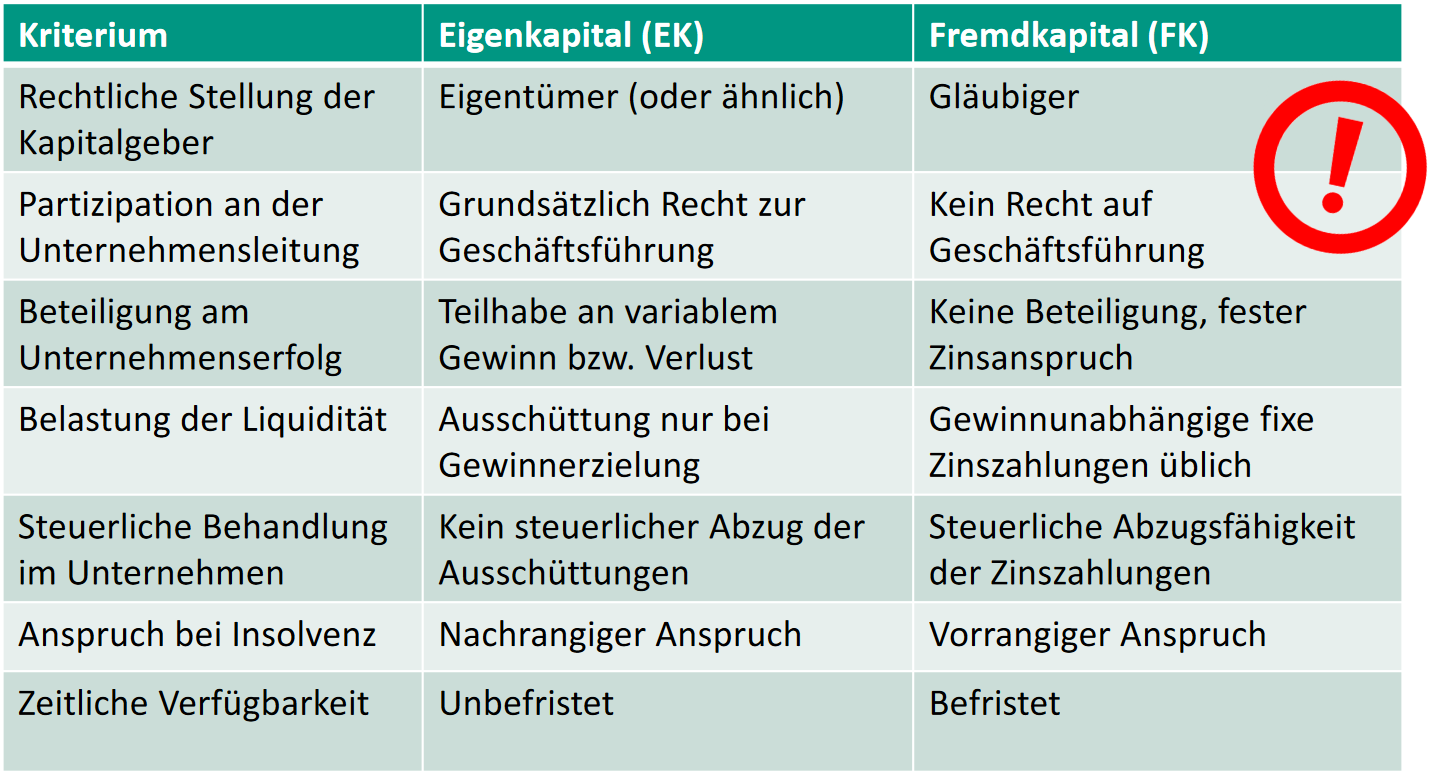
\includegraphics[width=0.8\textwidth]{images/ef-capital.png}
\end{center}

\textbf{Aktien}: Grundkapital einer Aktiengesellschaft wird in Aktien aufgeteilt und bildet neben Gewinnrücklagen das Eigenkapital. 
Diese können gehandelt werden und besitzen keine begrenzte Laufzeit.

\textbf{Stammaktien}:
\begin{itemize}
	\item Recht auf Anteil am Bilanzgewinn (\textbf{Dividende})
	\item Recht auf Anteil am Liquidationserlös
	\item Teilnahme, Rederecht, Stimmrecht auf Hauptversammlung
	\item Recht zur Stellung von Anträgen
	\item Auskunftsrecht
	\item Recht auf Bezug junger Aktien
\end{itemize}
\bigskip
\textbf{Vorzugsaktien}: Bestimmte Rechte kommen hinzu oder fallen weg (z.B. höhere Dividenden, mehr/weniger Stimmen)\\

\textbf{Kapitalbeschaffung durch Börsengang} (IPO, Initial Public Offering):
\begin{center}
	\includegraphics[width=0.75\textwidth]{images/börsengang.png}
\end{center}

\textbf{IPO-Phänomene}:
\begin{itemize}
	\item \textbf{Underpricing}: Bookbuildingpreis liegt meist deutlich unter dem ersten Handelskurs
	\item \textbf{Zyklizität}: Viele (wenige) IPOs in ökonomisch guten (schlechten) Zeiten
	\item \textbf{Kosten des Börsengangs}: Hohe Transaktionskosten für Unternehmen
	\item \textbf{Langfrist-Performance}: 3-5 Jahre nach IPO fällt meist eher durchschnittlich aus
\end{itemize}
\bigskip
\textbf{Kapitalbeschaffung durch Kapitalerhöhung}:
\begin{itemize}
	\item \textbf{Ordentliche Kapitalerhöhung}: Ausgabe von jungen Aktien zur Beschaffung neuen Eigenkapitals
	\item \textbf{Bedingte Kapitalerhöhung}: Kapitalerhöhung durch Umtausch-/Bezugsrecht\\ $\rightarrow$ Höhe ungewiss
	\item \textbf{Genehmigtes Kapital}: Ermächtigung des Vorstandes Eigenkapital zu emittieren, Kapital kann innerhalb dieses Zeitraums ohne Hauptversammlung erhöht werden 
	$\rightarrow$ Zeitpunkt ungewiss
\end{itemize}
\bigskip
\textbf{Auswirkung der Dividendenzahlung auf Aktienkurs}:
